\chapter*{工学启研第一期：如何写好学术邮件}

\section{活动简介}

“工学启研”是工学院学生会学术实践部面向本科生发起的系列分享活动，主要关注本科生科研训练、保研与留学申请中的实际问题。活动会持续收集同学和老师的反馈，围绕大家在学习和发展阶段遇到的困惑，提供更有针对性的经验分享。

第一期活动的主题是“如何写好学术邮件”。本期邀请了23级硕士余锦仁学长和24级博士郎青林学长，分别从邮件写作、联系老师、参与本科生科研等角度，分享了自己的经验和思考。

\begin{figure}
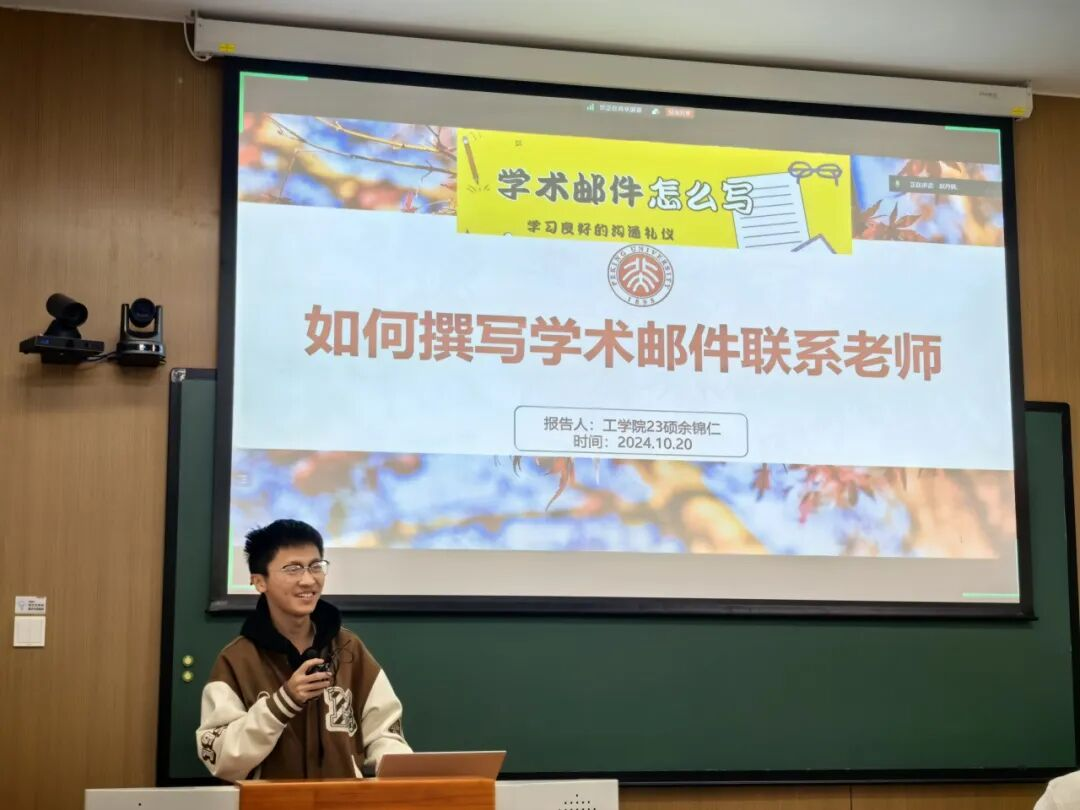
\includegraphics[width=0.92\linewidth]{assets/event-academic-email-lecture.jpg}
\caption{讲座现场：如何撰写学术邮件联系老师}
\end{figure}

\begin{figure}
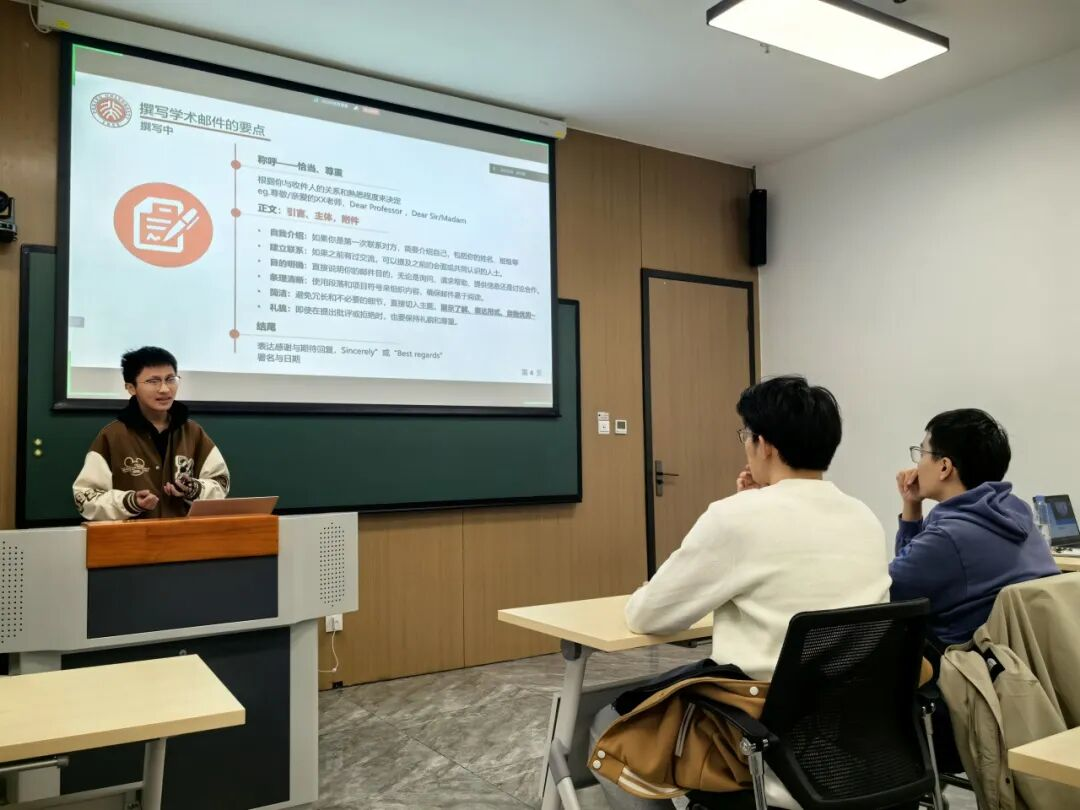
\includegraphics[width=0.92\linewidth]{assets/event-academic-email-audience.jpg}
\caption{余锦仁学长分享邮件写作经验}
\end{figure}

\section{余锦仁：把学术邮件写清楚、写得体}

\subsection{为什么学术邮件值得认真准备}

学术邮件可能出现在保研升学、本研入组、咨询建议、获取推荐信和寻找研究机会等场景中。它通常是老师或研究团队第一次了解你的窗口，因此邮件不需要追求华丽的文采，但需要让对方快速知道“你是谁、为什么联系、希望对方做什么”。

\subsection{发送前：先做充分调查}

写邮件之前，建议先列出与自己的兴趣和专业方向匹配的老师或研究团队，阅读对方近期的论文和出版物，了解最近关注的研究问题。充分调查有助于判断联系是否合适，也能让邮件中的自我介绍和联系理由更加具体。

\subsection{正文：信息完整而且有条理}

余锦仁学长结合自己在推免申请中使用过的邮件案例，介绍了几个关键环节：

\begin{enumerate}
\item 邮件主题应直接反映主要内容，避免空着，也不要使用模糊或过于随意的表述。
\item 开头使用恰当、尊重的称呼，并清楚介绍自己的年级、专业等必要信息。
\item 在正文中明确说明写信目的，并用简洁、有条理的语言交代与对方研究方向的关联。
\item 结尾表达感谢和对回复的期待，正确署名；涉及教务或财务等事务时，还应再次写明姓名和学号。
\end{enumerate}

\subsection{发送后：及时跟进，也要接受没有回复}

发送前应再次检查收件人、附件、称呼和关键信息，确认内容没有遗漏。学长建议，条件允许时优先使用学校提供的 edu 邮箱发送，并关注对方是否已经查收，在合适的时间进行一次礼貌的跟进。

对于没有回复的邮件，需要结合导师名额、招生安排以及对方是否拥有录取决定权等情况判断下一步行动。学长还按照常见的回复类型，分享了不同情况下的应对策略。

\subsection{不同联系路径的参考}

最后，余锦仁学长提供了个人自荐、通过第三方推荐以及跨专业联系时的邮件模板和案例，帮助大家把前面的原则落实到具体表达中。

\begin{figure}
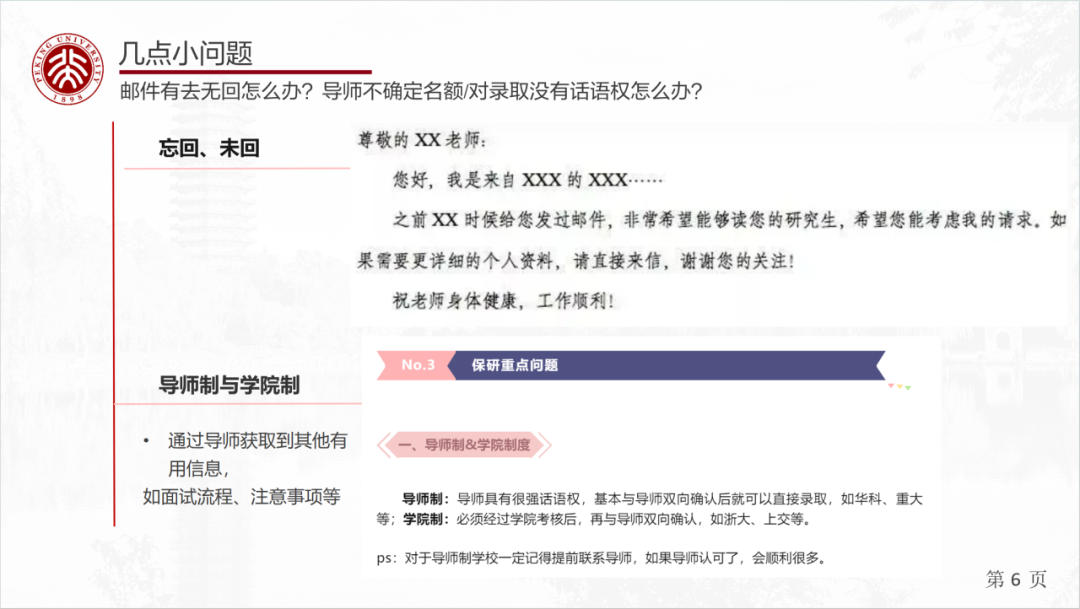
\includegraphics[width=0.92\linewidth]{assets/event-academic-email-example.png}
\caption{讲座中的邮件回复案例}
\end{figure}

\section{郎青林：科研邮件与本科生科研}

\subsection{科研邮件首先是功能性文字}

郎青林学长认为，科研邮件的首要功能是清晰传达信息，而不是展示华丽文采。邮件如果结构混乱、信息不足或过于冗长，容易给收件人留下不好的第一印象；写作时应始终站在收件人的角度，帮助对方快速理解你的身份、来意和诉求。

\begin{figure}
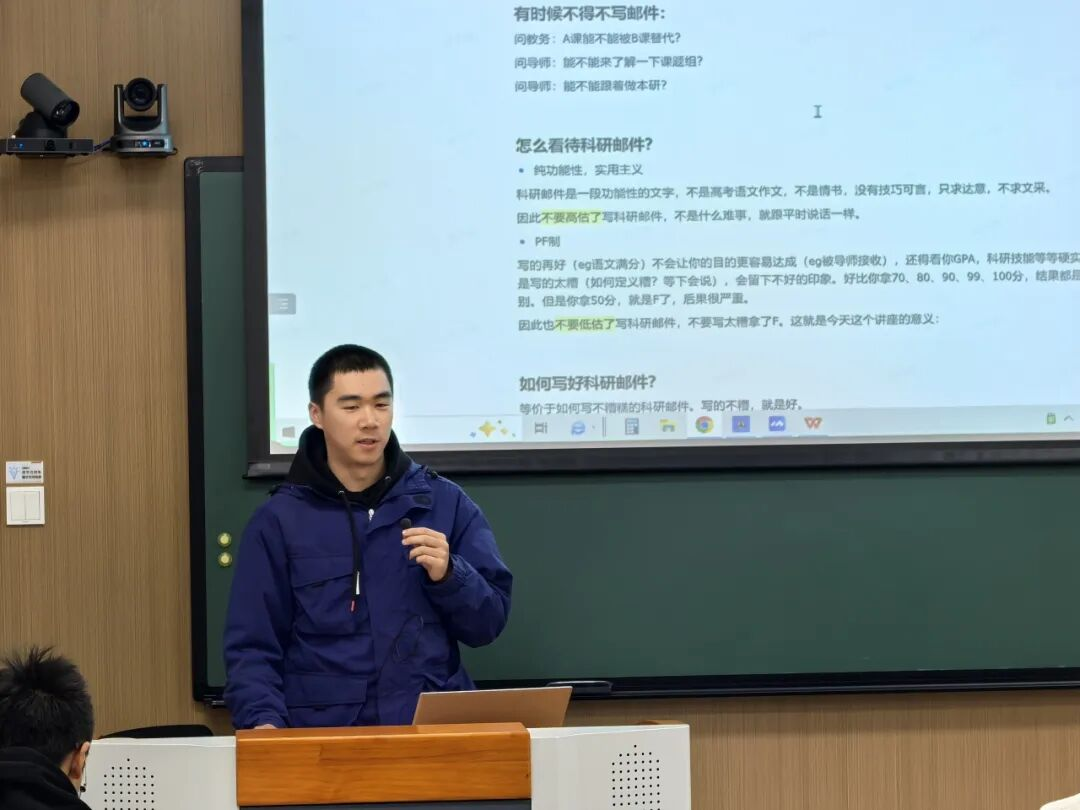
\includegraphics[width=0.92\linewidth]{assets/event-academic-email-lang.jpg}
\caption{郎青林学长分享科研邮件与本科生科研经验}
\end{figure}

他再次强调了几个细节：主题要直接反映邮件内容，不能留空；开头要说明自己的身份；结尾要再次写明姓名和学号（如果事务需要）；正文提供足够信息的同时，尽量保持简短；称呼和语气要礼貌、得体。

\subsection{邮件往来的几个惯例}

学长还分享了几条容易被忽略的邮件习惯：

\begin{itemize}
\item 客套一次即可，后续回复通常可以省略重复的问候和落款。
\item 不给他人增加无效邮件，例如教务问题已经得到明确回答时，不必为了表示感谢而专门再发一封邮件。
\item 使用换行来区分段落，保持邮件格式清晰，不要用连续空格代替段落结构。
\end{itemize}

为了帮助大家建立直观认识，郎青林学长以联系老师加入研究项目为例，展示了一封邮件模板，并再次提醒大家在写作时进行换位思考。

\subsection{如何理解本科生科研项目}

在介绍本研项目的基本情况后，郎青林学长建议大家根据自己的学习余力，选择合适的时间开始本科生科研。他将本研概括为两个重要功能：一是帮助同学测试自己是否对科研感兴趣，二是帮助同学在持续合作中建立与老师、团队之间的联系。这两点都可以帮助大家更早了解科研，并辅助判断未来的升学和发展方向。

\subsection{保持过程导向的心态}

本研更看重参与和积累的过程，而不是立刻得到一个“漂亮”的结果。遇到困难和挑战是科研训练中的常态，建议大家保持积极、稳定的心态，同时把专业课程学习放在基础位置，在保证学业质量的前提下参与科研。

\section{延伸阅读}

下面是本期活动中推荐的文章和资料，适合在写邮件、了解本科生科研或准备升学申请时继续阅读：

\begin{itemize}
\item \href{https://mp.weixin.qq.com/s/tjWFu6cLGwFmV1P91v8n7w}{张海霞：同学，注意邮件格式啊！}
\item \href{https://mp.weixin.qq.com/s/fwuviFt3tKGyfcXokMVTcg}{郎青林：本研、本科生心态}
\item \href{https://mp.weixin.qq.com/s/ap1fRs7ow2gxftS7byXAew}{高涵：保研}
\item \href{https://mp.weixin.qq.com/s/D-J4XQhenURe5ER0wwwmyw}{欧阳姝雨：跨专业保研}
\item \href{https://mp.weixin.qq.com/s/bN1ak8ItBLVLdy5ansyXZQ}{张艺馨：出国}
\item \href{https://mp.weixin.qq.com/s/kPczi0jLFKu8NW0hnZJqBw}{张宇辰：出国}
\end{itemize}

\section{写在最后}

一封好的学术邮件不在于辞藻复杂，而在于准备充分、信息清楚、表达尊重。希望这次分享能帮助大家在第一次联系老师、寻找科研机会或准备升学申请时少一些犹豫，多一份从容。
